 \documentclass[oneside,a4paper,12pt]{pictreport}
\usepackage{dirtree}
\usepackage{enumitem}
\usepackage{amsmath}
\usepackage{listings}
%\usepackage[table,xcdraw]{xcolor}
\usepackage{graphicx}
\usepackage{multirow}
\usepackage{enumitem}
\setlist[enumerate]{itemsep=0mm}


\lstset{basicstyle=\ttfamily,
  showstringspaces=false,
  commentstyle=\color{red},
  keywordstyle=\color{blue}
}
%\usepackage{showframe}
%\hoffset = 8.9436619718309859154929577464789pt
%\voffset = 13.028169014084507042253521126761pt
\usepackage{enumitem}
\setlist{parsep=0pt,listparindent=\parindent} %


\fancypagestyle{plain}{%
  \fancyhf{}
  \fancyfoot[C]{PICT, Department of Computer Engineering, 2017}
  \fancyfoot[R]{\thepage}
}
\pagestyle{fancy}
\fancyhead{}
\renewcommand{\headrulewidth}{0pt}
\footskip = 0.625in
\cfoot{}
\rfoot{}

\usepackage[hidelinks]{hyperref}
\usepackage{tikz}
\usetikzlibrary{arrows,shapes,snakes,automata,backgrounds,petri}

\usepackage{tabularx}

\usepackage[nottoc,notlot,notlof,numbib]{tocbibind}
\usepackage[titletoc]{appendix}
\usepackage{titletoc}
\renewcommand{\appendixname}{Annexure}
\renewcommand{\bibname}{REFERENCES}

\setcounter{secnumdepth}{5}
\usepackage{float}
\usepackage{subcaption}
\usepackage{multirow}

\usepackage[ruled,vlined]{algorithm2e}

\begin{document}

\picttitlepage{SENTIMENT ANALYSIS USING ORIGINAL AND REVERSED REVIEWS}{Kaushik S. Hande}{}{Prof. A. G. Phakatkar}

%\companycertificate{BEHAVIORAL ASSESSMENT OF INTERNAL AND EXTERNAL CANDIDATES OF MULTIPLE ORGANIZATIONS USING SENTIMENT ANALYSIS AND EMOTION MINING}{Sagar S. Patil}{}{Mr. Vijay Kumbhar}{Mr. Vijay Kumbhar}{}

\pictcertificate{SENTIMENT ANALYSIS USING ORIGINAL AND REVERSED REVIEWS}{Kaushik S. Hande}{}{Prof. A. G. Phakatkar}{}





\setcounter{page}{0}
\frontmatter
\cfoot{PICT, Department of Computer Engineering, 2017}
\rfoot{\thepage}
\pagenumbering{Roman}
\pictack{SENTIMENT ANALYSIS USING ORIGINAL AND REVERSED REVIEWS}{Kaushik S. Hande}{}{}

\listoffigures 
\listoftables
		
\begin{pictabstract}
Bag of words is used for modeling in machine learning algorithms. 
However, BOW is not able to handle negation well
because of its fundamental deficiencies . Many ways are used
to handle the problem of negation which results into polarity
shift . They require either knowledge about language constructs
or extra human interventions which eventually increases the
complexity. In this paper, a data expansion technique, called dual
sentiment analysis (DSA), is used to address the polarity shift
problem due to negation in sentiment classification. Original and
reversed training reviews are used for learning in a sentiment
classifier and prediction is done on test reviews.

\end{pictabstract}



% \maketitle
\tableofcontents
\mainmatter



\titleformat{\chapter}[display]
{\fontsize{16}{15}\filcenter}
{\vspace*{\fill} \bfseries\LARGE\MakeUppercase{\chaptertitlename}~\thechapter}
{1pc}
{\bfseries\LARGE\MakeUppercase}
[\thispagestyle{empty}\vspace*{\fill}\newpage]





\setlength{\parindent}{11mm}
\chapter{SYNOPSIS}


\section{Dissertation Title}
SENTIMENT ANALYSIS USING ORIGINAL AND REVERSED REVIEWS

%\section{Sponsorship}
%Webonise Lab, Pune.

%\section{External Guide} 
%Mr. Vijay Kumbhar

\section{Internal Guide}
Prof. A. G. Phakatkar



\section{Problem Statement}
\label{sec:problem_def}
"To make use of the original and reversed review samples in pairs for training a
statistical classifier and make predictions."

\section{Objectives}
\begin{itemize}
    \item To obtain reversed reviews from each corresponding original reviews.
    \item To train the classifiers  using these reviews.
    \item To obtain the predictions of labels(positive review or negative review) for test data.
\end{itemize}

\section{Hypothesis}

Polarity shift causes accuracy of classifier to decrease.
We assume that original review and corresponding opposite review can be used together to increase the accuracy of 
review class label prediction and to avoid the problem caused due to polarity shift.

\section{Relevant Mathematics Associated with Dissertation}

\subsection{Mathematical Model}

%\begin{equation*}
$S=\{s,e,I,O,fmain|\phi\}$\\ 
%\end{equation*}
where,\\
s = start state\\
e = end state\\
I = Inputs to the system\\
I = \{x,x${'}$,y,$y{'}$,D,D${'}$\}\\
where,\\
x = original sample\\
x${'}$ = reversed sample\\
y $\in$ \{0,1\} = The class label of the original sample\\
y${'}$ = \(1-y\) = The class label of the reversed sample\\
$
D = {(x_i,y_i )}_{i=1}^{n}$ = original training set\\
$ D{'}= {(x_i{'},y_i{'} )}_{i=1}^{n}$ = The reversed training set\\
O = Output \\
O = \{ p(x),p(x${'}$),p(x,x${'}$)\}\\
where\\
p(x) = Prediction for the original sample\\
p(x${'}$) = Prediction for the reversed sample\\
p(x,x${'}$) = Dual prediction based on a pair of sample\\
$f_{main} =\{f_{reverse},f_{classifier}\}$\\
$f_{reverse} =$ function for reversing the corresponding each review\\
$f_{classifier} =$ classifier for the prediction of class of review


\subsection{Metrics for Performance Evaluation}
Several statistical measures are used for performance evaluation - 
\begin{itemize}
\item Accuracy-is the proximity of measurement results to the true value.
\begin{equation}
\frac{TP + TN}{TP + TN + FP + FN}
\end{equation}
\item Sensitivity- measures the proportion of positives that are correctly identified
\begin{equation}
\frac{TP}{TP + FN}
\end{equation}
\item Specificity- measures the proportion of negatives that are correctly identified 
\begin{equation}
\frac{TN}{TN + FP}
\end{equation}
\item Positive predictive value- are the proportions of positive results in statistics and diagnostic tests 
\begin{equation}
\frac{TP}{TP + FP}
\end{equation}
\item Negative predictive value- are the proportions of negative results in statistics and diagnostic tests 
\begin{equation}
\frac{TN}{TN + FN}
\end{equation}
\end{itemize}

\chapter{TECHNICAL KEYWORDS}
\section{Area of Dissertation}
Natural language processing, machine learning, sentiment analysis, opinion mining.

\section{ACM Keywords}
\begin{enumerate}[label=\Alph*]
    \item Information Systems
    \begin{enumerate}[label*=.\arabic*]
    \item Information Retrievals
    \begin{enumerate}[label*=.\arabic*]
        \item Retrieval tasks and goals
        \begin{enumerate}[label*=.\arabic*]
            \item Sentiment analysis
            \item Clustering and classification
        \end{enumerate}
        \end{enumerate}
    \end{enumerate}
    \item Computing methodologies
        \begin{enumerate}[label*=.\arabic*]
            
            \item Machine learning
            \begin{enumerate}[label*=.\arabic*]
                \item Supervised learning by classification
                \begin{enumerate}[label*=.\arabic*]
                    \item Multinomial Naive Bayes
                    \item Random Forest
                    \item Support Vector Machines
                \end{enumerate}
            \end{enumerate}
        \end{enumerate}
    \end{enumerate}
\chapter{INTRODUCTION}

\section{Dissertation Idea}

\par Sentiment is an attitude, thought, or judgement prompted by feeling. Sentiment analysis 
is also known as opinion mining, it involves studing of people’s sentiments towards 
certain entities. Internet is a resourceful place with respect to sentiment information. From a
perspective of a user, people are able to express their views through various social media,
such as forums, micro-blogs, or online social networking sites.

\par With the advent of Web 2.0 techniques,
users started prefering to share their opinions on the Web. These user-generated and 
sentiment-rich data are valuable to many applications like 
credibility analysis of news sites on the Web, recommendation system, business and 
government intelligence etc. At the same time, it brings
urgent need for detecting overall sentiment inclinations of
documents generated by users, which can be treated as a
classification problem. Sentiment analysis includes several
subtasks  which have seen a great deal of attention in recent years:
\begin{enumerate}
 \item To detect whether a given document is subjective or objective.
  \item To Identify whether given subjective document express a positive opinion or a negative opinion.
  \item To determine the sentiment strength of a document,
such as strongly negative, weakly negative, neutral, weakly
positive and strongly positive.
\end{enumerate}

In this work we are focusing on second subtask.

\par Besides individuals on social media marketers also need to monitor all media for information related to their brands
whether it’s for public relations activities, fraud violations, or competitive intelligence.
Thus, aside from individuals, sentiment analysis is also the need of companies which are anxious to understand how
their products and services are perceived by the public.

\par The dominating text representation method in
both supervised and 
semi supervised sentiment
classification is known as the bag-of-words (BOW)
model, which is difficult to meet the requirements
for understanding the review text and dealing with
complex linguistic structures such as negation. For
example, the BOW representations of two opposite
reviews ``It works well'' and ``It doesn't work well''
are considered to be very similar by most statistical
learning algorithms.The two sentiment opposite texts are considered to be very similar by the
BOW representation. This is exactly why standard machine learning algorithms often
fail under the circumstance of polarity shift due to negation in the sentences of the review text.

\par Several approaches have been proposed in the literature
to address the polarity shift problem .They require either knowledge about language constructs or
extra human interventions which eventually increases the complexity in classification of sentiment.  Such
high-level dependency on external resources makes the systems 
difficult to be widely used in practice. There were also
some efforts to address the polarity shift problem with the
absence of extra annotations and linguistic knowledge. However, results are still far from satisfactory.
\section{Motivation of Dissertation}
Polarity shift is a kind of linguistic phenomenon which can reverse the sentiment polarity of the text. Negation is
the most important type of polarity shift. For example, by adding a negation word “don’t” to a positive text “I like
this book” in front of the word “like”, the sentiment of the this book” in front of the word “like”, the sentiment of the
text will be reversed from positive to negative. However,the two sentiment-opposite texts are considered to be
very similar by the BOW representation. This is the main reason why standard machine learning algorithms often
fail under the circumstance of polarity shift.


\chapter{LITERATURE SURVEY}

We studied the related work on sentiment analysis and
polarity shift.

\section{Sentiment Analysis and Polarity Shift}
\hspace{1.1cm}According to the levels of granularity, tasks in sentiment
analysis can be divided into four categorizations: document-
level, sentence-level, phrase-level, and aspect-level sentiment analysis.
\par 
For document and sentence-level sentiment classification, 
there are two main types of methods in the literature:
term-counting and machine learning methods. In term-
counting methods, the overall orientation of a text is
obtained by summing up the orientation scores of content
words in the text, based on manually-collected or external
lexical resources [38], [39]. In machine learning methods,
sentiment classification is regarded as a statistical 
classification problem, where a text is represented by a 
bag-of-words; then, the supervised machine learning algorithms
are applied as classifier [35]. Accordingly, 
the way to handle polarity shift also differs in the two types of methods.
\par
The term-counting methods can be easily modified to
include polarity shift. One common way is to directly
reverse the sentiment of polarity-shifted words, and then
sum up the sentiment score word by word [4], [16], [17],
[37]. Compared with term counting methods, the machine
learning methods are more widely discussed in the 
sentiment classification literatures. However, it is relatively
hard to integrate the polarity shift information into the
BOW model in such methods. For example, Das and
Chen [6] proposed a method by simply attaching “NOT”
to words in the scope of negation, so that in the text “I
don’t like book”, the word “like” becomes a new word “like-NOT”. Yet Pang et al. [35] reported that this method only
has slightly negligible effects on improving the sentiment
classification accuracy.
\par




\section{Gap Identification Through Literature Survey}

The following table shows the literature survey about different techniques of sentiment analysis used for classification. 

\renewcommand{\arraystretch}{1.0}
\begin{center}
\begin{table}[h!]
\caption{Literature Survey} 
\begin{tabular}{|l|l|l|l|}
\hline
No. & Reference                                                              & Techniques                                                                & Description                                                                 \\
\hline
1   & \begin{tabular}[c]{@{}l@{}}Dual Sentiment Analysis:\\ Considering Two sides of \\ 
one review\end{tabular}
  & \begin{tabular}[c]{@{}l@{}}Support vector machine\\(SVM), Naive bayes,\\ Logistic Regression \end{tabular}   
         & \begin{tabular}[c]{@{}l@{}}Dual training and \\
Dual Prediction \\technique is used.\end{tabular}                                                                                                                                                                                         \\
\hline
2   & \begin{tabular}[c]{@{}l@{}}Thumbs up?Sentiment \\
Classification using\\
Machine learning\\
algorithms\end{tabular} 
 & \begin{tabular}[c]{@{}l@{}}Learning algorithms\\
and n-gram model\end{tabular}                      
            & \begin{tabular}[c]{@{}l@{}}Classify the dataset\\
using different\\
machine.\end{tabular}                                                                                                                                                                      \\
\hline
3   & \begin{tabular}[c]{@{}l@{}}Classification of \\sentiment
reviews using\\
N-gram machine \\learning
approach\end{tabular}                 & \begin{tabular}[c]{@{}l@{}}Support Vector Machine\\
Naive Bayes \end{tabular}            & \begin{tabular}[c]{@{}l@{}}Converting text\\
reviews into numeric\\
matrices using\\
countvectorizer and\\
TF-IDF\end{tabular}                                                                                                                                                          \\
\hline
4   & \begin{tabular}[c]{@{}l@{}}Thumbs up or \\thumbs
down? Semantic \\orientation
applied to \\unsupervised
classification \\of reviews\end{tabular}                                          & \begin{tabular}[c]{@{}l@{}}Unsupervised
learning \\algorithm for\\
classifying a \\review\end{tabular}                                                         & \begin{tabular}[c]{@{}l@{}}A specific unsupervised\\
learning technique \\based
on the\\
mutual information\end{tabular}                                                                                                                                                                                        \\
\hline
5   & \begin{tabular}[c]{@{}l@{}}Automatic Opinion \\polarity
Classification \\of movie\end{tabular} & \begin{tabular}[c]{@{}l@{}}Naive Bayes\\
And Markov Model \\(MM) \end{tabular}  & \begin{tabular}[c]{@{}l@{}} Accessed overall \\opinion
polarity(OvOp)\\
concept using \\machine
learning\\ algorithm\end{tabular}                                                                                                                                                 \\
\hline
6   & \begin{tabular}[c]{@{}l@{}}Dual Training and \\dual
prediction for\\ polarity
classification\end{tabular}                                                                                    & \begin{tabular}[c]{@{}l@{}} SVM and Naive Bayes\end{tabular}                                                           & \begin{tabular}[c]{@{}l@{}}Dual training and\\
dual prediction \\(DTDP)\end{tabular}                                                                                                                                                                          \\
\hline

7  & \begin{tabular}[c]{@{}l@{}}A 3D Hand Tracking\\ Design for Gesture\\ Control in Complex \\Environments\end{tabular}                                                                                & \begin{tabular}[c]{@{}l@{}}3D hand tracking design\end{tabular}                         & \begin{tabular}[c]{@{}l@{}}It segments hands \\out of entire image \\and also facilitates \\depth estimation of \\tracked hands in\\ real-time by dual \\camera systems.\end{tabular}                                                                                                                                                                      \\
\hline
8  & \begin{tabular}[c]{@{}l@{}}Hand tracking and \\Gesture Recognition\end{tabular}                                                                              & \begin{tabular}[c]{@{}l@{}}Kalman filter and\\
derived Scale Invariant \\Feature Transform (SIFT).\end{tabular}                  & \begin{tabular}[c]{@{}l@{}}It presents a method \\for tracking and \\recognizing hand\\ gestures by extracting \\ unique invariant \\features from gestures.\end{tabular}  \\          
\hline
\end{tabular}
\end{table}
\end{center}
\newpage
\renewcommand{\arraystretch}{1.0}
\begin{center}
\begin{table}[h!]
\begin{tabular}{|l|l|l|l|}
\hline
No. & Reference                                                              & Techniques                                                                & Description                                                                 \\
\hline
9  & \begin{tabular}[c]{@{}l@{}}Hand Position Tracking \\Using a Depth Image \\from a RGB-d Camera\end{tabular}                                               & \begin{tabular}[c]{@{}l@{}}RGB image based on \\the skin color
Hand \\Tracking \end{tabular}                                                      & \begin{tabular}[c]{@{}l@{}}The algorithms can be\\ used for natural user \\interfaces, the guidance of the\\end effector \\of an industrial robot\\ and hand segmentation.\end{tabular}
\\    
\hline
10 & \begin{tabular}[c]{@{}l@{}}Indian Sign Language \\Recognition: \\Database Creation, Hand \\Tracking and Segmentation\end{tabular}                       & \begin{tabular}[c]{@{}l@{}}YcbCr based skin \\color model \end{tabular}     & \begin{tabular}[c]{@{}l@{}}This algorithm works \\on motion tracking, \\edge detection and \\skin color detection.\end{tabular}          \\
\hline
\end{tabular}
\caption{Literature Survey} 
\end{table}
\end{center}

\chapter{PROBLEM DEFINITION AND SCOPE}

\section{Goals}
\begin{itemize}
\item Understanding existing sentiment analysis approaches.
\item Study corpus based, lexical based and semantic based techniques.
\item Understanding unigram, bigram, trigram and combination of them for modeling purpose.
\item Training the model with naive bayes, support vector machine, maximum entropy.
\item Applying this learned model to the test dataset.
\item Evaluating the results generated by classifiers.
\end{itemize}

\section{Objectives}

Please refer Chapter 1, Section 1.7 on Page 2

\section{Statement of Scope}
\begin{itemize}
\item Preprocessing the reviews
\item Classify reviews into two polarities.
\item Evaluate the classification accuracy by each classifier.
\end{itemize}

\section{Software Context}
\subsection{Scikit-learn} 
Scikit-learn (formerly scikits.learn) is a free software machine learning library for the Python programming language. It features various classification, regression and clustering algorithms including support vector machines, random forests, gradient boosting, k-means and DBSCAN, and is designed to interoperate with the Python numerical and scientific libraries NumPy and SciPy.

\subsection{NumPY}


NumPy is the fundamental package for scientific computing with Python. It contains among other things:
\begin{itemize}
\item A powerful N-dimensional array object
\item Sophisticated (broadcasting) functions
\item Tools for integrating C/C++ and Fortran code
\item Useful linear algebra, Fourier transform, and random number capabilities
\end{itemize}
Besides its obvious scientific uses, NumPy can also be used as an efficient multi-dimensional container of generic data. Arbitrary data-types can be defined. This allows NumPy to seamlessly and speedily integrate with a wide variety of databases.

\subsection{Natural language toolkit}
NLTK is a leading platform for building Python programs to work with human language data. It provides easy-to-use interfaces to over 50 corpora and lexical resources such as WordNet, along with a suite of text processing libraries for classification, tokenization, stemming, tagging, parsing, and semantic reasoning, wrappers for industrial-strength NLP libraries, and an active discussion forum.

\subsection{Matplotlib}
Matplotlib is a Python 2D plotting library which produces publication quality figures in a variety of hardcopy formats and interactive environments across platforms. Matplotlib can be used in Python scripts, the Python and IPython shell, the jupyter notebook, web application servers, and four graphical user interface toolkits. You can generate plots, histograms, power spectra, bar charts, errorcharts, scatterplots, etc., with just a few lines of code.

\chapter{DISSERTATION PLAN}

\section{Purpose of the Document}
This document specifies and estimates various risks associated with this project and states how they are handled. It also states the project plan in terms of task and their dependency.

\section{Technical Constraints}
\begin{itemize}
\item To build a classification module that distributes data and execution among spark executors.
\item To fetch candidate's tweets in a CSV format and store it in Alluxio.
\end{itemize}

\section{Dissertation Estimates}
\subsection{Reconciled Estimates}
\subsubsection{Cost Estimates}
No cost is required for tools and software as open source softwares are used.
\subsubsection{Time Estimates}
Calendar time required: 11 months.
\subsubsection{Dissertation Resources}
\begin{itemize}
\item People : Single Person
\item Hardware resources used are mentioned in Chapter 6, Section 6.5 on Page XX
\item Software resources used are mentioned in Chapter 6, Section 6.6 on Page XX
\end{itemize}

\section{Risk Management}
This section discusses dissertation risks and the approach to managing them.
\subsection{Risk Identification}
For risks identification, review of scope document, requirement specifications and schedule is done. Answers to questionnaire revealed some risks. Following risk identification questionnaire has been referred.
\begin{itemize}
\item Are requirements fully understood by the software engineering team and its customers?
\item Have customers been involved fully in the definition of requirements?
\item Do end-users have realistic expectations?
\item Does the software engineering team have the right mix of skills?
\item Are project requirements stable?
\item Is the number of people on the project team adequate to do the job?
\item Do all customer/user constituencies agree on the importance of the project and on the requirements for the system/product to be built?
\end{itemize}

\subsection{Risk Analysis}
The risks for the dissertation are analyzed within the constraints of time and quality. Risk can be as follows:

\begin{itemize}
\item Out of memory error, while creating model and training the model.
\item Review text contains unrecognized characters.
\item Out of memory error, while predicting on the test dataset.
\end{itemize}
Please refer Table 5.1, 5.2 and 5.3 for detail description.

\renewcommand{\arraystretch}{1.5}
\begin{table}[h!]
\caption{Risk Table}
\begin{tabular}{|l|l|l|l|l|l|}
\hline
\textbf{ID} & \textbf{Risk Description} & \textbf{Probability} & \multicolumn{3}{c|}{\textbf{Impact}}                                         \\ \hline
            & \textbf{}                 & \textbf{}            & \textbf{Schedule} & \textbf{Quality} & \textbf{Overall} \\ \hline
1           & Out of Memory             & High                & Low                      & High                    & High                    \\ \hline
2           & Unrecognized characters            & Low               & Medium                   & High                    & Medium                  \\ \hline
3           & Out of Memory         & Low               & Medium                   & High                    & High                    \\ \hline
\end{tabular}
\end{table}

\begin{table}[h!]
\centering
\caption{Risk Probability Definitions}
\begin{tabular}{|l|l|l|}
\hline
\textbf{Probability} & \textbf{Value}                   & \textbf{Description} \\ \hline
High                 & Probability of the occurrence is & \textgreater 75\%    \\ \hline
Medium               & Probability of the occurrence is & 26\% - 74\%          \\ \hline
Low                  & Probability of the occurrence is & 25\%                 \\ \hline
\end{tabular}
\end{table}

\begin{table}[h!]
\centering
\caption{Risk Impact Definitions}
\begin{tabular}{|l|l|l|}
\hline
\textbf{Impact} & \textbf{Value}    & \textbf{Description}                                                                                                                                        \\ \hline
Very High       & \textgreater 10\% & Schedule impact or Unacceptable quality                                                                                                                     \\ \hline
High            & 5\%-10\%          & \begin{tabular}[c]{@{}l@{}} Schedule impact or Some parts of \\ the project have low quality  \end{tabular}                                                                                              \\ \hline
Low             & \textless5\%      & \begin{tabular}[c]{@{}l@{}}Schedule impact or Barely noticeable \\degradation in quality Low Impact on schedule or\\ Quality can be incorporated\end{tabular} \\ \hline
\end{tabular}
\end{table}

\subsection{Overview of Risk Mitigation, Monitoring and Management}
Please refer Table 5.4, 5.5 and 5.6 for detail description.

\begin{table}[h!]
\centering
\caption{Risk 1}
\label{my-label}
\begin{tabular}{|l|l|}
\hline
\textbf{Risk ID}          & 1                                                    \\ \hline
\textbf{Risk Description} & Out of memory error, when training Model \\ \hline
\textbf{Category}         & Configuration                                        \\ \hline
\textbf{Source}           & Software Requirement Specification Document          \\ \hline
\textbf{Probability}      & High                                                 \\ \hline
\textbf{Impact}           & High                                                 \\ \hline
\textbf{Response}         & Mitigate                                             \\ \hline
\textbf{Strategy}         & Changing number of features resolves this issue.     \\ \hline
\textbf{Risk Status}      & Occurred and Resolved                                \\ \hline
\end{tabular}
\end{table}


\begin{table}[h!]
\centering
\caption{Risk 2}
\label{my-label}
\begin{tabular}{|l|l|}
\hline
\textbf{Risk ID}          & 2                                                                     \\ \hline
\textbf{Risk Description} & Unreconized characters                                     \\ \hline
\textbf{Category}         & Configuration                                                         \\ \hline
\textbf{Source}           & Software Requirement Specification Document                           \\ \hline
\textbf{Probability}      & Low                                                               \\ \hline
\textbf{Impact}           & Low                                                                \\ \hline
\textbf{Response}         & Mitigate                                                              \\ \hline
\textbf{Strategy}         & Convert all characters into unicode format \\ \hline
\textbf{Risk Status}      & Occurred and Resolved                                                 \\ \hline
\end{tabular}
\end{table}
\begin{table}[h!]
\centering
\caption{Risk 3}
\label{my-label}
\begin{tabular}{|l|l|}
\hline
\textbf{Risk ID}          & 3                                           \\ \hline
\textbf{Risk Description} & Out of memory error, when predicting    \\ \hline
\textbf{Category}         & Development Environment                     \\ \hline
\textbf{Source}           & Software Requirement Specification Document \\ \hline
\textbf{Probability}      & Low                                     \\ \hline
\textbf{Impact}           & Low                                        \\ \hline
\textbf{Response}         & Mitigate                                    \\ \hline
\textbf{Strategy}         & Using sparse matrix to represent text                \\ \hline
\textbf{Risk Status}      & Occurred and Resolved                       \\ \hline
\end{tabular}
\end{table}
\newpage
\section{Staff Organization}

\subsection{Team Structure}
\begin{itemize}
    \item Internal Guide : Prof. A. G. Phakatkar
    %\item External Guide : Mr. Vijay Kumbhar
    \item Student : Kaushik S. Hande 
\end{itemize}

\subsection{Management Reporting and Communication}
The progress of dissertation is reported once in a month.
\section{Dissertation Schedule}
\subsection{Dissertation Task Set}
Major tasks in the Dissertation stages are - 
\begin{itemize}
\item Installing the required libraries in python environment.
\item Creating bag of words model from text reviews.
\item Understand and build a document classifier.
\item Test the classifier on test dataset.
\item To find accuracy, precision, recall and other evaluation measures.
\end{itemize}
Please refer Annexure B, Table B.1 on Page 66 for all Dissertation Tasks.
\subsection{Task Network}
\begin{figure}[!h]
\centering
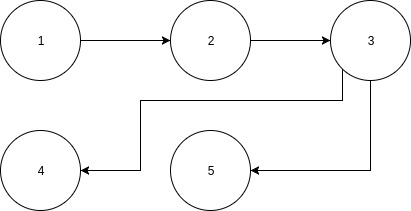
\includegraphics[width=5.5in,height=3.2in]{task.jpg}
\caption{Task Network}
\end{figure}
\newpage
\subsection{Timeline Chart}
\begin{figure}[!h]
\centering
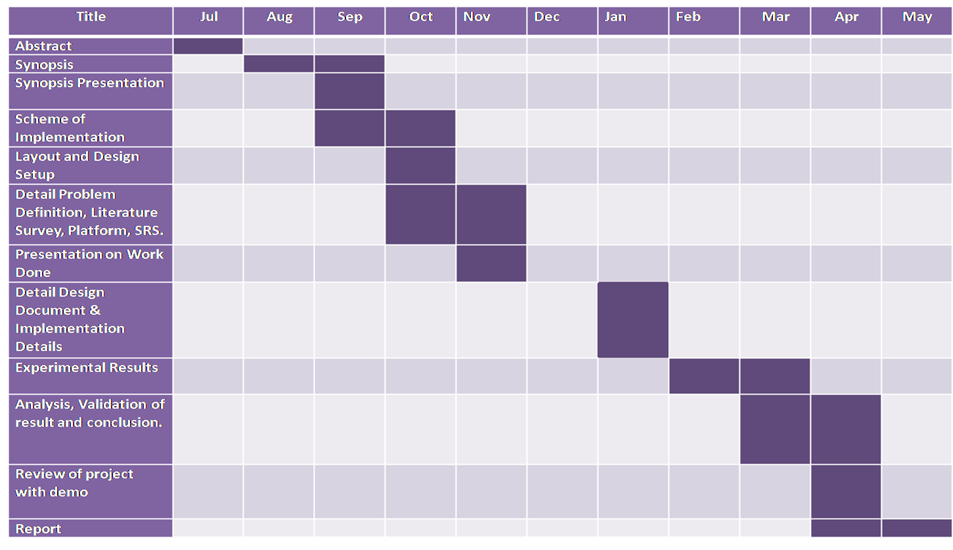
\includegraphics[width=5.5in,height=5.5in]{timeline.png}
\caption{Timeline Chart}
\end{figure}

\chapter{SOFTWARE REQUIREMENT SPECIFICATION}

\section{Introduction}
The aim of this document is to specify the software requirements for classification of movie reviews.

\section{Purpose and Scope of the Document}
The purpose of the document is to enlist various software requirements to build the system. This document has functional and non-functional requirements for the software being developed.

\section{Overview of Responsibilities of Developer}
The responsibilities of a developer includes gathering of information about the classification libraries, that can be used to design and develop the system to categorize movie reviews. The developer’s responsibilities include: 
\begin{itemize}
\item Planning for dissertation (Scheduling) 
\item Designing of system (High Level Design Document)
\item Coding of system (Implementation)
\item Testing of system (Test Cases)
\end{itemize}

\section{Product Overview}
System builds classifier models for classification of reviews. Different functionality of the system are : 

\begin{itemize}
\item Candidate Registration - It shows a registration page that candidate uses to registers for one of the organizations.
\item Candidate Data Downloading - It allows a Product Admin to download candidate's tweets from Twitter.
\item Candidate Profiling - Profiles are formed for specific candidate after analyzing tweets in the form of column graph. It shows percentage of emotional and polarity categories scores. Scores are shown year-wise, month-wise and day-wise.
\item Candidate Comparison - It allows Product Admin to compare two candidates with respect to their emotional and polarity scores achieved. Comparison graphs of candidates are shown year-wise, month-wise and day-wise.
\item Managing Candidate's Details and Data - It allows Product Admin to delete candidate's data or details or both.
\end{itemize}
\section{Hardware Resources Used}
\subsection{Software Requirements}
\begin{itemize}
				\item Python 2.7.6 
				\item Rstudio Version 0.99.893 
				\item R version 3.3.2
				\item Operating Systems:
					\begin{itemize}
						\item Windows XP, 7, 8, 10
						\item Linux(Any flavor)
						\item Mac OS 
					\end{itemize}
\end{itemize}
\subsection{Hardware Requirements}
			\begin{itemize}
				\item Intel(R) Core(TM) i3 CPU @ 2.90GHz or later, width : 64 bits
				\item Memory : 4 GB DDR3 or more
				\item Capacity : 1697MHz or more
				\item Cores : 4 or more
				\item PCI Express Gigabit Ethernet Controller, Size: 100Mbit/s, Capacity: 1Gbit/s, Width: 64 bits
				\item Hard Disk : 500 GB (EXT4 Primary/Logical Partition)
			\end{itemize}
		
\newpage

\section{Functionality}
\begin{itemize}
\item Download movie reviews from imDb dataset.
\item Import the moview review dataset into python environment using csv package.

\item Convert the text reviews into matrix form.
\item Remove the stopwords from reviews.
\item Show positive and negative polarity score for test reviews.


\item Compare classifiers for accuracy of classification.
\end{itemize} 

\section{Input}
\begin{itemize}
\item Dataset that consists of movie reviews and their corresponding labels.
\item List of stopwords which play no role in classification.
\end{itemize}


\section{Output}
\begin{itemize}
\item Classification of each test review into positive or negative.
\item Percentage of accuracy achieved in classification.
\item Comparison of accuracies obtained by each classifier.
\end{itemize}

\section{Major Constraints}

\begin{itemize}
\item To store movie reviews as input in csv file format.
\item To execute classifiers in configured environment.
\item To train the model for polarity classification.
\end{itemize}

\section{Applications}
\begin{itemize}
\item Businesses and organisations which require consumer opinions to do with products they market and services they produce.
\item Individuals who make decisions to purchase products or services based upon word of mouth or on-line reviews, or to find public opinion, e.g. concerning politics or local issues.
\item On-line advertising where in social media, an organisation may place an advertisement in response to a favourable review of a product, or a rival product could be advertised upon receipt of a bad review
\item Opinion retrieval for general searches of opinions
\item HR Analytics.
\end{itemize}

\section{Usage Scenario}
A use case represents a particular functionality of a system. Hence, use case diagram is used to describe the relationships among the functionalities and their internal/external actors. This section provides various usage scenarios for the system to be developed.

\subsection{User Profiles}
Actors of the system are Candidate, Product Administrator, Storage System, Database System and Web Interface.
\begin{itemize}
    \item \textbf{Candidate} : Actor registers for a specific organization giving twitter URL and other details to Database using Web Interface.
    \item \textbf{Product Administrator} : Actor manages registers candidates, downloads tweets of a candidate, manages several behavioral assessment tests, profiles and compares candidates.
    \item \textbf{Storage System} : Actor stores tweets of candidates downloaded by Product Administrator.
    \item \textbf{Database System} : Actor stores emotional, polarity scores and other details of candidates.
    \item \textbf{Web Interface} : Actor displays candidate's emotional and polarity graphs according to year, month and day. It also allows Product Admin to download candidate's data and manage behavioral assessment tests.  
\end{itemize}
\newpage
\subsection{Use Cases}
Table 7.1 gives Use Cases for system to be developed.
\renewcommand{\arraystretch}{1.0}
\begin{table}[h]
\centering
\caption{Use Cases}
\label{my-label}
\begin{tabular}{|l|l|l|l|l|}
\hline
\textbf{Sr. No.} & \textbf{Use Case}                                                 & \textbf{Descriptions}                                                                                                                                                                                                    & \textbf{Actors}                                                                                                          & \textbf{Assumptions}                                                                                                    \\ \hline
1                & \begin{tabular}[c]{@{}l@{}}Candidate \\ Registration\end{tabular} & \begin{tabular}[c]{@{}l@{}}Candidate has to \\ registers for a \\ specific organization \\ giving necessary\\ details and saved \\ to Database.\end{tabular}                                                             & \begin{tabular}[c]{@{}l@{}}Candidate,\\ Database\\ System\end{tabular}                                                   & \begin{tabular}[c]{@{}l@{}}Provided\\ details \\ are correct\end{tabular}                                               \\ \hline
2                & \begin{tabular}[c]{@{}l@{}}Candidate Data\\ Download\end{tabular} & \begin{tabular}[c]{@{}l@{}}Product Admin \\ fetches candidate's\\  details from\\  database, Extract \\ screen name\\ from Twitter URL, \\ downloads candidate's \\ data and store it \\ in storage system.\end{tabular} & \begin{tabular}[c]{@{}l@{}}Candidate,\\ Database System, \\ Storage System,\\ Product\\ Admin\end{tabular}               & \begin{tabular}[c]{@{}l@{}}Data\\ is \\ downloaded\\  properly.\end{tabular}                                            \\ \hline
3                & \begin{tabular}[c]{@{}l@{}}Candidate \\ Comparison\end{tabular}   & \begin{tabular}[c]{@{}l@{}}Product Admin \\ chooses\\ two candidates\\ for comparison\\  based \\ on emotional and\\ polarity values.\end{tabular}                                                                       & \begin{tabular}[c]{@{}l@{}}Candidate,\\ Database System, \\ Product Admin, \\ Web Interface\end{tabular}                 & \begin{tabular}[c]{@{}l@{}}Comparison\\ between \\ two candidates \\ are \\ shown in the \\ form of graph.\end{tabular} \\ \hline
4                & \begin{tabular}[c]{@{}l@{}}Candidate \\ Profiling\end{tabular}    & \begin{tabular}[c]{@{}l@{}}Candidate are \\ profiled\\ based on set\\ of rules defined\\ by Product Admin.\end{tabular}                                                                                                  & \begin{tabular}[c]{@{}l@{}}Candidate,\\ Database System, \\ Product Admin, \\ Web Interface\end{tabular}                 & \begin{tabular}[c]{@{}l@{}}Profile\\ results are \\ displayed\\  in the form of \\ column graph.\end{tabular}           \\ \hline
5                & System                                                            & \begin{tabular}[c]{@{}l@{}}Overall \\ system\\ description\end{tabular}                                                                                                                                                  & \begin{tabular}[c]{@{}l@{}}Candidate,\\ Product Admin,\\ Database System,\\ Web Interface,\\ Storage System\end{tabular} & \begin{tabular}[c]{@{}l@{}}System\\ is\\ functional\end{tabular}                                                        \\ \hline
\end{tabular}
\end{table}
\newpage
\subsection{Use Case Views}
\subsubsection{Candidate Registration}
\begin{figure}[h!]
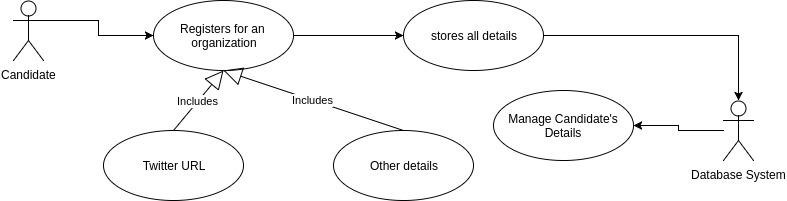
\includegraphics[width=5.2in,height=1.5in]{UseCase1.jpg}
\caption{Use Case : Candidate Registration}
\end{figure}
\subsubsection{Candidate Data Download}
\begin{figure}[h!]
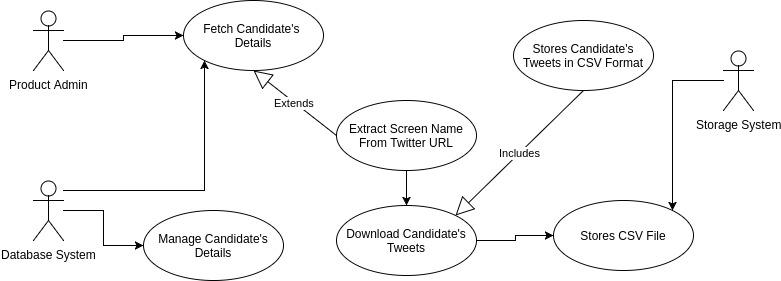
\includegraphics[width=5.2in,height=2.0in]{UseCase2.jpg}
\caption{Use Case : Candidate Data Download}
\end{figure}
\newpage
\subsubsection{Candidate Comparison}
\begin{figure}[h!]
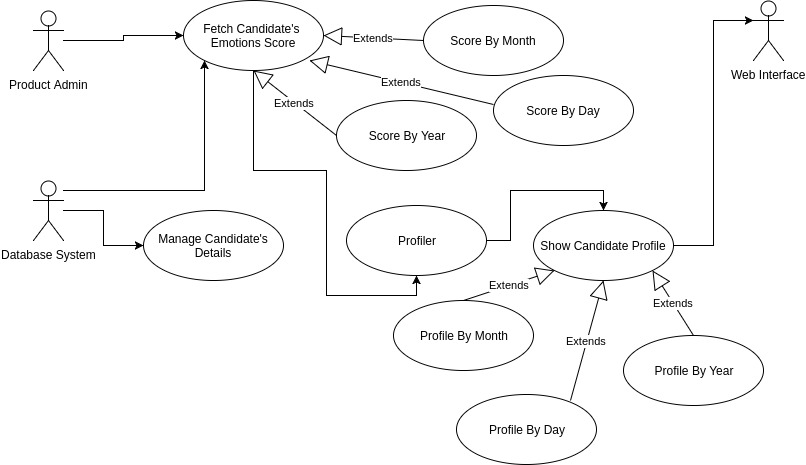
\includegraphics[width=5.2in,height=3.5in]{UseCase3.jpg}
\caption{Use Case : Candidate Comparison}
\end{figure}
\subsubsection{Candidate Profiling}
\begin{figure}[h!]
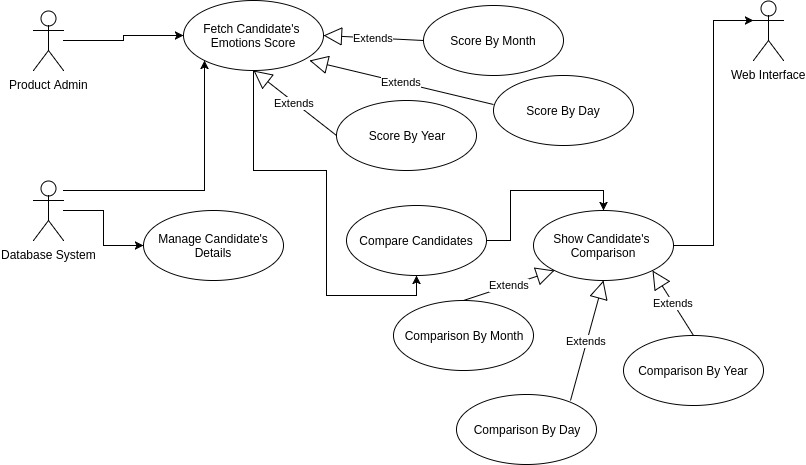
\includegraphics[width=5.2in,height=3.5in]{UseCase4.jpg}
\caption{Use Case : Candidate Profiling}
\end{figure}
\newpage
\subsubsection{System Use Case}
\begin{figure}[h!]
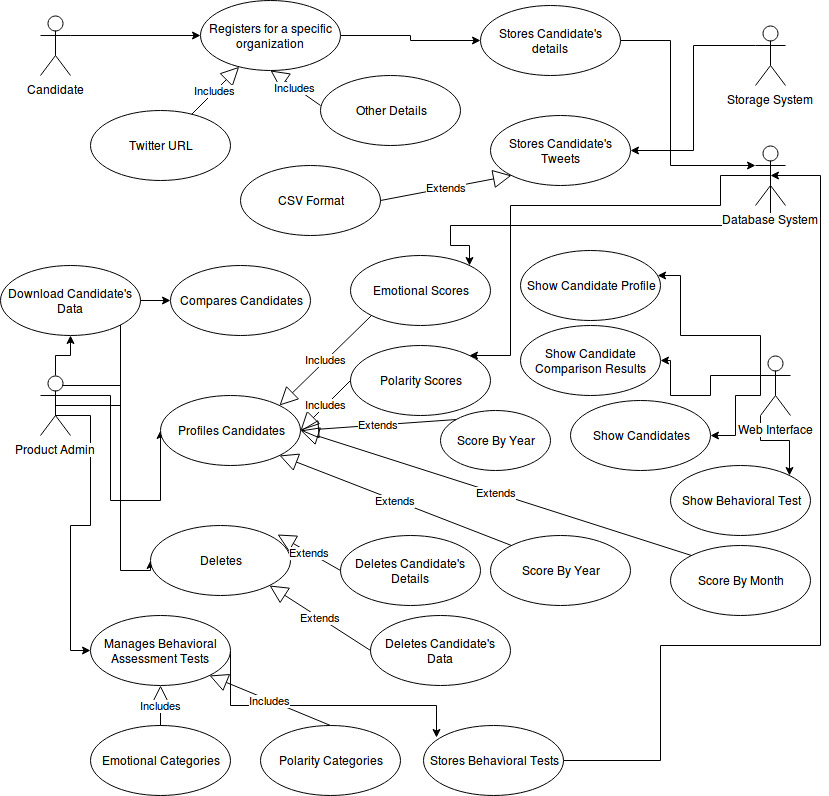
\includegraphics[width=5.2in,height=4.4in]{SystemUseCase.jpg}
\caption{Use Case : Overall System}
\end{figure}
\newpage
\section{Behavioral Model and Description}
This section contains details about events and associated behaviour of the system which is shown using diagram below.

\subsection{Activity Diagram}
Activity diagram is a flow chart to represent the flow form one activity to another activity. The activity can be described as an operation of the system. The control flow is drawn from one operation to another. This flow can be sequential, branched or concurrent. The purpose of activity diagrams is to capture the dynamic behaviour of the system.\\\\
\textbf{Description} : As shown in figure 7.6, Product Administrator downloads candidate's tweets from Twitter for analysis. Tweets are stored in a CSV format in Alluxio data storage. For analysis to take place, candidate's download status is check. If it is true, load candidate's CSV file and proceed with analysis else download candidate's tweets. For document classification, initially model existence is checked. If it exists, then load model for document classification else proceed with training phase. The training phase consists of document preprocessing, feature extraction and saving model in Alluxio. Classifier uses this trained model for document classification. Candidates are profiled and compared based on their document classified into emotional and polarity categories.
\begin{figure}[h!]
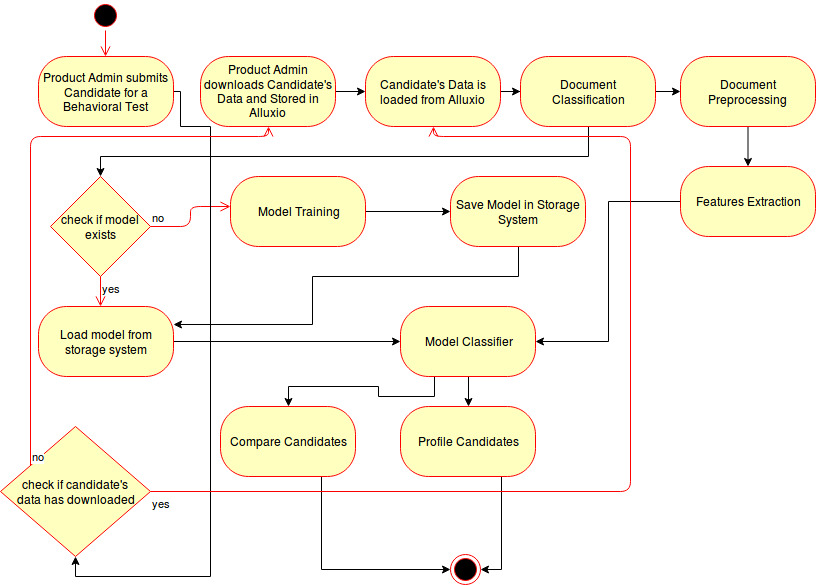
\includegraphics[width=5.0in,height=4.0in]{Activity.jpg}
\caption{Activity Diagram}
\end{figure}
\newpage
\section{Functional Model and Description}
This section describes data flow diagrams (DFD) of the proposed system. There are three types of DFDs explained in the section. These diagrams explain the system in brief.

\subsection{Data Flow Diagram}
\subsubsection{Level 0 Data Flow Diagram}
In the level 0 DFD as shown in figure 7.7, Candidates registers into Behavioral Assessment System. System performs analysis and generates reports for a registered candidate. They are displayed to Product Admin.\\
\begin{figure}[h!]
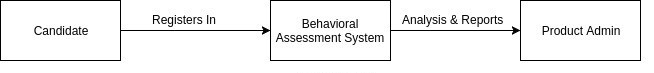
\includegraphics[width=4.5in]{DFD-0.jpg}
\caption{Level 0 DFD}
\end{figure}

\subsubsection{Level 1 Data Flow Diagram}
In the level 1 DFD as shown in figure 7.8, Candidate's tweets are fetched from Twitter by Product Admin using Web Interface. Tweets are stored in Alluxio for storage. They are retrieved by Web Application modules for analysis and report generation.\\
\begin{figure}[h!]
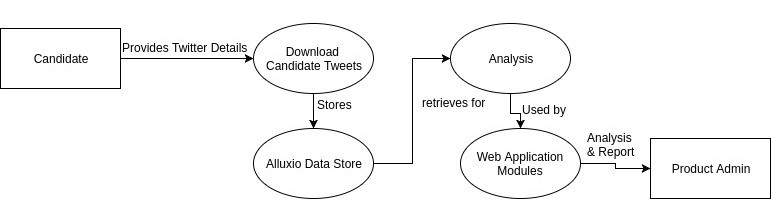
\includegraphics[width=4.5in]{DFD-1.jpg}
\caption{Level 1 DFD}
\end{figure}

\subsubsection{Level 2 Data Flow Diagram}
In the level 2 DFD as shown in figure 7.9, Candidate's tweets are retrieved from Alluxio Data Storage and preprocessed. Features are extracted for Classification. It classifies tweets of a candidate to emotional and polarity categories. Candidate are profiled and compared based on these categories. Profile and comparison results are displayed to Product Admin using Web Interface.\\
\begin{figure}[h!]
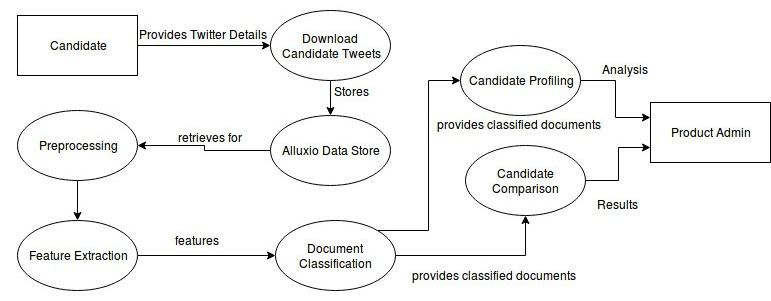
\includegraphics[width=4.5in]{DFD-2.jpg}
\caption{Level 2 DFD}
\end{figure}
\\
\section{Non-Functional Requirements}
\subsection{Availability}
Required libraries must be installed and loaded in the python environment with the required configurations. Dataset must be downloaded from specified url \cite{dataset}.

\subsection{Scalability}
The system should be scalable to classify reviews even if the training and test data are increased. System can comfortably handle 
reviews dataset upto 25000 reviews.

\subsection{Performance}
The system must be interactive and delays involved must be less. There should be no immediate delays for every action and response of the system. Training time increases as the training data increases. It takes 4 to 5 seconds in training the dataset. Training increases further when bigram and trigram models are used.


\subsection{Usability}
The system should be easy to handle and process requests efficiently. System's functions are designed to use with ease and provide results. Results are presented in the form of graphs and are easy to comprehend.

\subsection{Reliability}
The system should efficiently analyze movie reviews entirely and give correct classification result. It should be reliable to perform 
classification effectively on any review dataset.
\subsection{Maintainability and Changeability}
The system is made up of different independent modules that can be modified to correct faults, improve performance or other attributes, or adapt to a changed environment. System can be improved for new features and will be able to include new requirements.

\chapter{DETAILED DESIGN DOCUMENT}

\section{Introduction}
This document specifies the design that is used to fetch candidate tweets in CSV format, classifies individual tweets into emotion and polarity categories, profiles candidates based on predefined rules and predict future behavior of candidate.

\section{Behavioral Modeling}
Candidate's tweets are classified into emotional and polarity categories. Over the course of candidate's social media presence, profile deviates that forms a iterative behavioral model.
\begin{itemize}
    \item \textbf{Emotional Categories}
    \begin{itemize}
        \item Anger
        \item Disgust
        \item Joy
        \item Love
        \item Fear
        \item Sadness
        \item Surprise
    \end{itemize}
    \item \textbf{Polarity Categories}
    \begin{itemize}
    \item Positive
    \item Negative
    \item Offensive
    \end{itemize}
\end{itemize}
Candidate's tweets are collected and classified based on these categories. They are profiled and compared based on emotional and polarity categories.
\newpage
\section{Architectural Design}
\begin{figure}[!h]
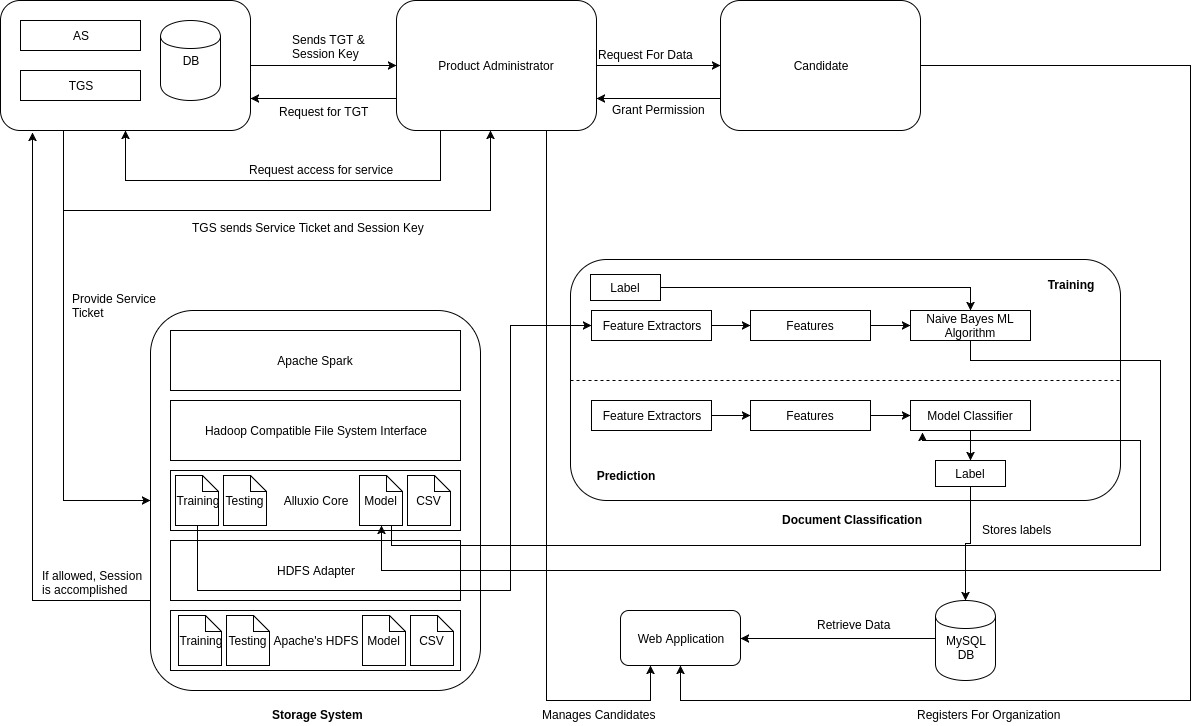
\includegraphics[width=5.7in,height=4.0in]{Architecture.jpg}
\caption{Proposed System Architecture}
\end{figure}
Figure 7.1 shows architectural design of proposed system. Following are important components in the system :
\begin{itemize}
\item Storage System : Alluxio, memory centric storage system is used as main storage system which stores in-memory data. Apache's HDFS is used as an underFS storage system. Candidate's CSV files, trained models, testing and training dataset is stored in Alluxio.
\item Computation Framework : Apache's Spark is used for computations. Document classifier is built in Spark. It access candidate's CSV, trained model files from Alluxio. Spark's Mlib is used for training Naive Bayes model which is stored in Alluxio after training.
\item Document Classifier : First, Naive Bayes model is trained by training dataset of emotional and polarity categories and saved in Alluxio. After training, prediction stage occurs. It access candidate's CSV file from Alluxio and classifies document on each candidate's tweet. Predicted labels on each tweet is stored in MySQL database with year, month and day.
\item Candidate registers for specific organization using web application, providing twitter details. Product Administrator access web application to download candidate's tweets from Twitter, manages candidates, profiles and compares candidates. 
\item Kerberos is  used for mutual authentication between storage system components and document classifier. It consists of Authentication Server, Database and Ticket Granting Service. Product Administrator requests Key Distribution Center for a valid ticket before submitting Spark job. If no valid ticket found, operation is not permitted. With only valid ticket, candidate's tweets are analyzed.  
\end{itemize}
\section{Class Design}
It is a static diagram that represents the static view of an application. It is not only used for visualizing, describing, and documenting different aspects of a system but also for constructing executable code of the software application. It describes the attributes and operations of a class and also the constraints imposed on the system.\\\\
\textbf{Description} : In figure 8.2, modules and their relationships are shown. Document classifier used for classifying candidate's tweets takes user identifier of candidate and candidate's CSV location in Alluxio as an input. Product Administrator fetches candidate's tweets from Twitter in a CSV format and store the file in Alluxio. Candidate's CSV file location is saved into database for further processing. After document classification, candidates can be profiled and compared based on their emotional and polarity categories. For both modules, results are displayed by year, month and day.
\begin{figure}[h!]
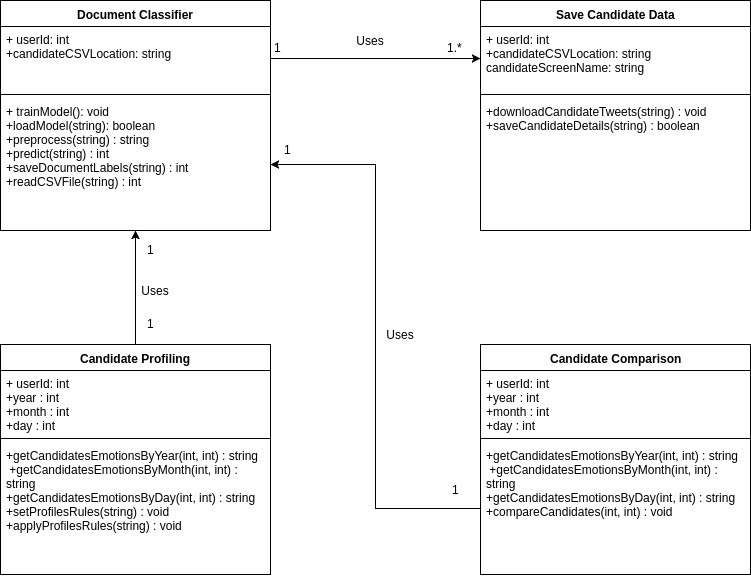
\includegraphics[width=4.5in,height=4.0in]{Class.jpg}
\caption{Class Diagram}
\end{figure}
\newpage
\section{Component Design}
It is used to model the physical aspects of a system. It is also used to visualize the organization and relationships among components in a system. It does not describe the functionality of the system but it describes the components used to make those functionalities.\\\\
\textbf{Description} : Figure 8.3 describes primary components of the system. A web application provides candidate's tweets to be fetched and candidates are profiled and compared functionality to Product Administrator. Product Admins are authenticated first before using any of the functionality. To download tweets of a specific candidate, he/she must register for that organization. Tweets are stored in Alluxio data storage in CSV format. Data storage is accessed by Spark application for fetching candidate's tweets for preprocessing and document classification. 
\begin{figure}[h!]
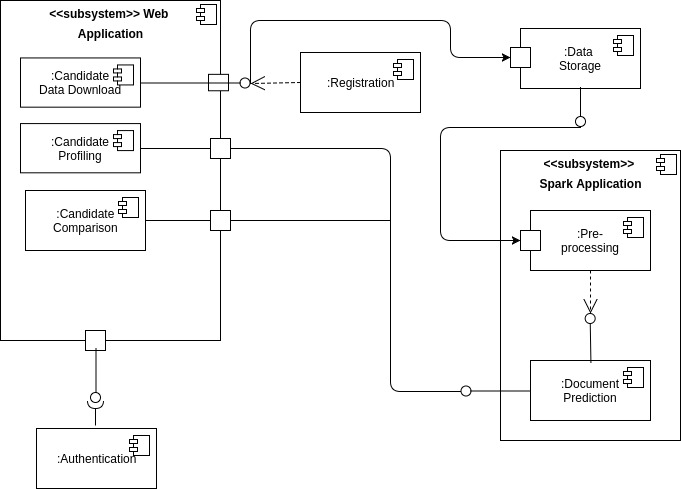
\includegraphics[width=5.2in,height=4.2in]{component.jpg}
\caption{Component Diagram}
\end{figure}
\section{Deployment Design}
 It is used visualize the topology of the physical components of a system, where the software components are deployed. It describes the static deployment view of a system, consisting of nodes and their relationships.\\\\
 \textbf{Description} : In figure 8.4, Web application designed in Laravel PHP runs on Apache Tomcat Server. Process component of Symphony is used to run spark application. 4-Node cluster is formed for spark application execution. It requires data from Alluxio data storage system. Alluxio is specifically compiled for Spark for data access. Web application retrieves candidate's emotional and polarity scores from database.
\begin{figure}[h!]
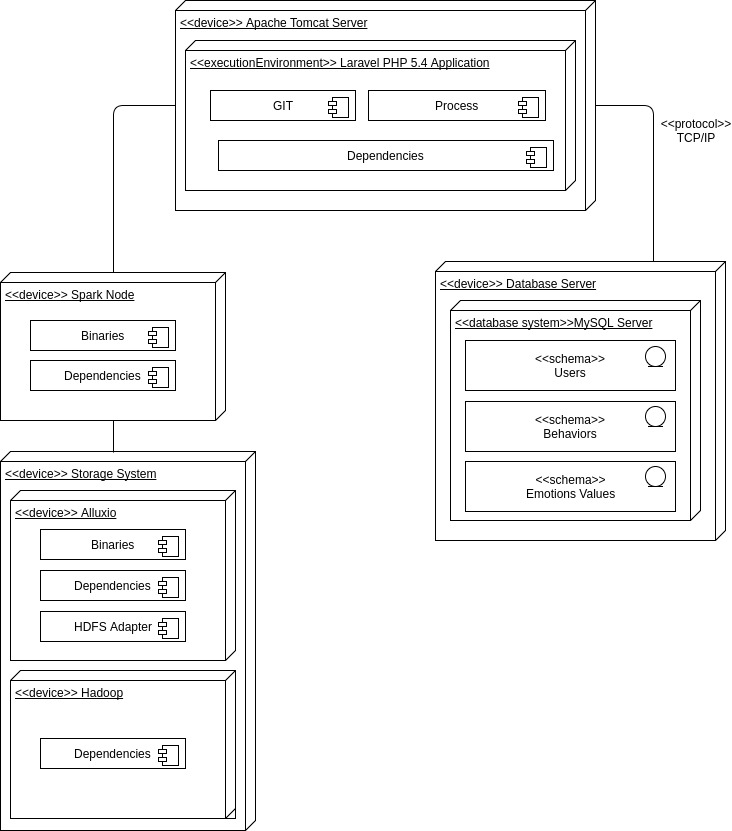
\includegraphics[width=5.2in,height=4.2in]{Deployment.jpg}
\caption{Deployment Diagram}
\end{figure}

\chapter{IMPLEMENTATION DETAILS}
\section{Introduction}
This section describes implementation of the system, required libraries and dependencies needed for components of the system and use of implementation strategy.
\section{Algorithm}
\subsection{Document Classification}

\textbf{Input} : Candidate's CSV file and Unique Identifier. \\
\textbf{Output} : Candidate's tweets classified into emotional and polarity categories. \\\\
Initialize numFeatures to 10000 \\
Initialize emotionalTrainingDataPath to /emotion-training \\  
Initialize polarityTrainingDataPath to /polarity-training \\
Initialize emotionModel to /emotion-model \\
Initialize polarityModel to /polarity-model \\
Input candidateCSVLocation \\
Input candidateUserId \\\\
If  emotionModel exists
    \par load emotionModel\\
Else
    \par load Category Data from emotionalTrainingDataPath
	\par transform Category Data using Hashing Transform for numFeatures
	\par attach label to Category Data
	\par save emotionModel to /emotion-model
	\par load emotionModel from /emotion-model\\
If  polarityModel exists
	\par load polarityModel \\
Else
	\par load Category Data from polarityTrainingDataPath
	\par transform Category Data using Hashing Transform for numFeatures
	\par attach label to Category Data
	\par save polarityModel to /polarity-model
	\par load polarityModel from /polarity-model\\
Read CSV file from candidateCSVLocation\\
While CSV file contains some rows
	\par Read Columns from CSV file
	\par Column 0 contains 'Date'
	\par Column 1 contains 'Actual Tweet'
	\par Split Column 0 into year, month and day
	\par Transform Column 1 using Hashing Transform for numFeatures
	\par Classify Column 1 with respect to emotionModel and get emotionLabel
	\par Save emotionLabel into database with year, month and day
	\par Classify Column 1 with respect to polarityModel and get polarityLabel
	\par Save polarityLabel into database with year, month and day

\subsection{Candidate Profiling}
\textbf{Input} : Candidate's User Identifier.\\
\textbf{Output} : Candidate Profiles\\\\
Input Candidate's User Identifier.\\
Retrieve years from Database based on UserId\\
Retrieve months from Database based on UserId\\
Retrieve days from Database based on UserId\\\\
\textbf{Calculate Percentage of Categories for all years}\\
Retrieve emotionsValues from Database based on UserId for all years\\
Retrieve polarityValues from Database based on UserId for all years\\\\
While candidate has emotion category and value in a year
	\par Calculate Total number of documents in a year
	\par Calculate Total number of document for a specific category
	\par Calculate Percentage for a specific category\\
While candidate has polarity category and value in a year
	\par Calculate Total number of documents in a year
	\par Calculate Total number of document for a specific category for a year
	\par Calculate Percentage for a specific category for a year\\\\
\textbf{Calculate Percentage of Categories for all months}\\
Retrieve emotionsValues from Database based on UserId for all months group by years\\
Retrieve polarityValues from Database based on UserId for all months group by years\\\\
While candidate has emotion category and value in a month for specific year
	\par Calculate Total number of documents in a month
	\par Calculate Total number of document for a specific category
	\par Calculate Percentage for a specific category for a month\\
While candidate has polarity category and value in a month for specific year
	\par Calculate Total number of documents in a month
	\par Calculate Total number of document for a specific category for a year
	\par Calculate Percentage for a specific category for a month\\\\
\textbf{Calculate Percentage of Categories for all days}\\\\
Retrieve emotionsValues from Database based on UserId for all days in a month for a specific year\\
Retrieve polarityValues from Database based on UserId for all days in a month for a specific year\\\\
While candidate has emotion category and value for all days in a month for specific year
	\par Calculate Total number of documents in a day
	\par Calculate Total number of document for a specific category
	\par Calculate Percentage for a specific category for a day\\
While candidate has polarity category and value for all days in a month for specific year
	\par Calculate Total number of documents in a day
	\par Calculate Total number of document for a specific category
	\par Calculate Percentage for a specific category for a day
\section{Modules}
\subsection{Candidate's Tweets Fetched From Twitter}
\begin{itemize}
\item This modules retrieves candidate's tweets from Twitter. Input to module is candidate's screen name. 
\item Every user in twitter has unique screen name which can be used to retrieve his/her tweets using Twitter APIs and OAuth. 
\item OAuth 2 is an authorization framework that enables application to obtain limited access to user accounts on an HTTP service such as Facebook and Twitter. 
\item A Twitter application is created, python module connects to Twitter application using consumer secret key and consumer key. Twitter application also generates access key and access secret key which decides validity of tweets access. Tweets are fetch and store it in CSV format. 
\item The CSV file of every candidate is pushed to Alluxio storage system. Python's Tweepy library is used for implementation of this module. 
\item A Product Administrator uses candidate data downloading functionality to trigger this module giving candidate's screen name as an input.
\end{itemize}
\subsection{Document Classification}
\begin{itemize}
\item This module takes candidate's CSV location in Alluxio and unique identifier as an input. 
\item This module is written in Scala and executes as an spark job on multi-node spark cluster. This means, spark job uses resources of multiple connected nodes for faster processing. 
\item Alluxio is memory centric distributed storage system that provides candidate's CSV file to spark job. Spark's Machine Learning library is used for  implementation of Naive Bayes Classifier. 
\item Initially, model is trained by training dataset that consists of emotional categories of 21429 records and polarity categories of 8797 records. Both models are saved to and loaded from Alluxio. 
\item Every candidate's tweet is classified into one of the emotional and polarity categories. A database insertion operation push classified documents along with user identifier to MySQL.
\end{itemize}

\subsection{Web Application}
Web application is designed and built in Laravel PHP 5.4. High charts is used for showing candidate results in the form of column graphs. There are different modules in web application - 
\begin{itemize}
\item Candidate Profiling : Module shows each candidate's emotional and polarity categories percentage year-wise, month-wise and day-wise.
\item Candidate Comparison : Two candidates are compared by emotional and polarity categories percentage. Results are shown year-wise, month-wise and day-wise.
\item Candidate Data Downloading Functionality : It enables product administrator to download tweets of a certain candidate. It uses Process component of Symphony to execute python script that fetches tweets from Twitter.
\item Storage Analyzer : It shows storage space used by candidate's CSV files, training and testing dataset and saved trained models in Alluxio. Alluxio's local file system commands are used to retrieve space occupied. 
Registration – It allows a candidate to register himself/herself to a certain organization. 
\item Assessment creation and deletion : Assessments are created, deleted and updated by product administrator. 
\end{itemize}

\section{Dataset}
\hspace{1.1cm}Dataset comprises of tweets from Twitter. It has to be collected for every candidate that needs to be assessed for behavioural assessment. There is significant latency and load on server in fetching such information of candidate using Twitter API.
\par After the dataset is collected, it needs to be stored in underFS storage layer. Movement of huge dataset to storage layer requires additional I/O writes and communication overhead. But, by using proposed system, writes operation to storage layer is significantly lesser.
\par For document classification, a training and testing dataset is required. Training records for emotional and polarity categories are mentioned in Table 9.1 and 9.2.

\renewcommand{\arraystretch}{1.5}
\begin{table}[h!]
\centering
\caption{Emotional Training Dataset}
\label{my-label}
\begin{tabular}{|l|l|}
\hline
\textbf{Emotion Category} & \textbf{Training Records} \\ \hline
Anger                     & 1572                      \\ \hline
Joy                       & 8276                      \\ \hline
Disgust                   & 761                       \\ \hline
Love                      & 216                       \\ \hline
Sadness                   & 3853                      \\ \hline
Surprise                  & 3912                      \\ \hline
Fear                      & 2839                      \\ \hline
\textbf{Total}            & \textbf{21429}            \\ \hline
\end{tabular}
\end{table}

\begin{table}[h!]
\centering
\caption{Polarity Training Dataset}
\label{my-label}
\begin{tabular}{|l|l|}
\hline
\textbf{Polarity} & \textbf{Training Records} \\ \hline
Positive          & 2007                      \\ \hline
Negative          & 4783                      \\ \hline
Disgust           & 2007                      \\ \hline
\textbf{Total}    & \textbf{8797}             \\ \hline
\end{tabular}
\end{table}


\section{Snapshots}

\chapter{TEST SPECIFICATION}

\section{Introduction}
This document explains the test plan and testing strategy for modules in a system. Following modules needs to be tested - 
\begin{itemize}
\item Fetching candidate's tweets from Twitter and store it in CSV format.
\item Classification of candidates in emotional and polarity categories.
\item Web application that sends requests, collect responses and act based on responses.
\end{itemize}

\subsection{Goals and Objectives}
\begin{itemize}
\item To validate candidate's tweets in a CSV after fetching it from Twitter.
\item To check accuracy of different document classifiers.
\item To validate predicted document labels of candidate's tweets.
\item To validate candidate's profiles and comparison results.
\item To validate execution distribution among multiple connected nodes.
\end{itemize}

\subsection{Statement of Scope}
Testing will be done on individual modules of a system. Testing will be carried out for several different candidates. Finally, system as a whole is tested for correctness of results. 

\subsection{Major Constraints}
Testing is done manually. For testing the accuracy of document classifiers, testing dataset is formed and used. Total number of multiple connected nodes is limited to four nodes.

\section{Test Plan}
\subsection{Modules to be Tested}
\begin{itemize}
\item Candidate's tweets fetched from Twitter module.
\item Candidate's tweets classification module.
\item Web Application.
\end{itemize}

\subsection{Testing Strategy}
\subsubsection{Unit Testing}
Unit testing has been done for all the individual modules. While doing unit testing different parameter has been considered and according to input to the system different output is recorded. After recording output of unit testing different solution are applied to pass the test. This is carried out as white box testing.
\begin{itemize}
\item To test candidate's tweets are fetched and stored in a CSV format.
\item To test classification module's effectiveness and prediction of document labels.
\item To test different classifier's accuracy.
\item To test candidate profiles and comparison's results. Result must be shown in the form of graph.
\item To test candidate's documents analysis occurs distributively, using resources of multiple connected nodes. 
\end{itemize}

\subsubsection{Integration Testing}
Once unit testing is complete for individual modules, all the modules are integrated together and tested for functional correctness. While doing integration testing, developer has kept in mind few constraints which need to be achieved in order to get desired results.
\begin{itemize}
\item Web application requests needs to be accepted by classification module and response back with predicted document labels for candidate's tweets.
\item Web application uses candidate's data download functionality to fetch candidate's tweets from Twitter and store it in Alluxio.
\item Web Application retrieves candidate's analysis results and forms a column b ar graph.
\item Candidates are compared for seven emotional categories and results are shown as a graph.
\end{itemize}

\subsubsection{Validation Testing}
Validation testing is carried out to test the entire work flow and input validation. This is carried out as a black box testing. In this project validation testing has been conducted on different modules.
\begin{itemize}
\item To validate candidate's tweets in a CSV after fetching it from Twitter.
\item To validate predicted document labels of candidate's tweets.
\item To validate candidate's profiles and comparison results.
\item To validate execution distribution among multiple connected nodes.
\end{itemize}

\subsubsection{System Testing}
\begin{itemize}
\item To test if all GUI elements are shown properly in a web interface.
\item To test if spark application is executed atomically using web interface.
\item To test if spark application is able to access data stored in Alluxio.
\item To test if Kerberos is integrated into Spark and Alluxio.
\end{itemize}

\subsubsection{GUI Testing}
Front End of the system is designed as web application, runs on local server. Data visualization is provided by High charts. \\
Following modules needs to be tested in a web application - 
\begin{itemize}
\item Candidate's data downloading functionality
\item Assessment creation and deletion
\item Storage Analyzer
\item Candidate's profiles
\item Candidates comparison 
\end{itemize}

\subsubsection{High Order Testing}
It includes carrying out performance testing by checking complete running time of document classification on multinode spark cluster.

\subsection{Test Procedure}
\subsubsection{Unit Testing}
\begin{table}[h!]
\centering
\caption{Unit Test Cases}
\begin{tabular}{|l|l|l|l|l|}
\hline
\textbf{Sr. No.} & \textbf{\begin{tabular}[c]{@{}l@{}}Test Case \\ Name\end{tabular}}               & \textbf{\begin{tabular}[c]{@{}l@{}}Test Case\\ Objective\end{tabular}}                                                                       & \textbf{\begin{tabular}[c]{@{}l@{}}Test Case\\ Input\end{tabular}}                        & \textbf{\begin{tabular}[c]{@{}l@{}}Test Case\\ Result\end{tabular}} \\ \hline
1                & Log In                                                                           & \begin{tabular}[c]{@{}l@{}}Product Admin should\\ be able to log in for\\ correct organization\\ only.\end{tabular}                          & \begin{tabular}[c]{@{}l@{}}Username \&\\ Password\end{tabular}                            & Pass                                                                \\ \hline
2                & \begin{tabular}[c]{@{}l@{}}View\\ Candidates\end{tabular}                        & \begin{tabular}[c]{@{}l@{}}Product Admin should \\ be able to view all\\ candidates registered\\ for organization.\end{tabular}              & \begin{tabular}[c]{@{}l@{}}Candidate's\\ Details\end{tabular}                             & Pass                                                                \\ \hline
3                & \begin{tabular}[c]{@{}l@{}}Create \\ Behavioral\\ Assessment\\ Test\end{tabular} & \begin{tabular}[c]{@{}l@{}}Product Admin should\\ be able to create\\ customized behavioral\\ test.\end{tabular}                             & \begin{tabular}[c]{@{}l@{}}Emotional and\\ polarity\\ categories's \\ values\end{tabular} & Pass                                                                \\ \hline
4                & \begin{tabular}[c]{@{}l@{}}Candidate\\ Registration\end{tabular}                 & \begin{tabular}[c]{@{}l@{}}Candidate should be\\ able to register for \\ specific organization.\end{tabular}                                 & \begin{tabular}[c]{@{}l@{}}Candidate's\\ Details\end{tabular}                             & Pass                                                                \\ \hline
5                & \begin{tabular}[c]{@{}l@{}}Manage \\ Candidate\\ Data\end{tabular}               & \begin{tabular}[c]{@{}l@{}}Product Admin should\\ be able to delete \\ candidate's records \\ and tweets stored in\\ CSV format\end{tabular} & \begin{tabular}[c]{@{}l@{}}Candidate's\\ User Identifier\end{tabular}                     & Pass                                                                \\ \hline
\end{tabular}
\end{table}
\subsubsection{Integration Testing}
\begin{table}[h!]
\centering
\caption{Integration Test Cases}
\begin{tabular}{|l|l|l|l|l|}
\hline
\textbf{Sr. No.} & \textbf{\begin{tabular}[c]{@{}l@{}}Test Case \\ Name\end{tabular}} & \textbf{\begin{tabular}[c]{@{}l@{}}Test Case\\ Objective\end{tabular}}                                                                                                    & \textbf{\begin{tabular}[c]{@{}l@{}}Test Case\\ Input\end{tabular}}                    & \textbf{\begin{tabular}[c]{@{}l@{}}Test Case\\ Result\end{tabular}} \\ \hline
1                & \begin{tabular}[c]{@{}l@{}}Candidate\\ Profiling\end{tabular}      & \begin{tabular}[c]{@{}l@{}}Product Admin\\ submits candidate's\\ tweets for profiling.\\ Emotional and polarity\\ scores must be generated\\ after analysis.\end{tabular} & \begin{tabular}[c]{@{}l@{}}Candidate's \\ Unique\\ Identifier\end{tabular}               & Pass                                                                \\ \hline
2                & \begin{tabular}[c]{@{}l@{}}Candidate\\ Comparison\end{tabular}     & \begin{tabular}[c]{@{}l@{}}Product Admin selects two\\ candidates for comparison.\\ Comparison occurs based on\\ emotional and polarity scores.\end{tabular}              & \begin{tabular}[c]{@{}l@{}}Unique User\\ identifier \\ of both candidates.\end{tabular} & Pass                                                                \\ \hline
\end{tabular}
\end{table}
\newpage
\subsubsection{Validation Testing}
\begin{table}[h!]
\centering
\caption{Validation Test Cases}
\begin{tabular}{|l|l|l|l|l|}
\hline
\textbf{Sr. No.} & \textbf{\begin{tabular}[c]{@{}l@{}}Test Case \\ Name\end{tabular}}                                 & \textbf{\begin{tabular}[c]{@{}l@{}}Test Case\\ Objective\end{tabular}}                                                                                   & \textbf{\begin{tabular}[c]{@{}l@{}}Test Case\\ Input\end{tabular}}                                  & \textbf{\begin{tabular}[c]{@{}l@{}}Test Case\\ Result\end{tabular}} \\ \hline
1                & \begin{tabular}[c]{@{}l@{}}Candidate\\ Data\\ Validation\end{tabular}                              & \begin{tabular}[c]{@{}l@{}}Candidate's details\\ are first validated\\ against rules set.\end{tabular}                                                   & \begin{tabular}[c]{@{}l@{}}Candidate's\\ details.\end{tabular}                                      & Pass                                                                \\ \hline
2                & \begin{tabular}[c]{@{}l@{}}Candidates\\ listing for\\ Behavioral\\ Assessment\\ Tests\end{tabular} & \begin{tabular}[c]{@{}l@{}}Candidates whose\\ tweets are fetched \\ should only appear \\ in list for test.\end{tabular}                                 & \begin{tabular}[c]{@{}l@{}}Candidate's\\ Twitter Data\\ Download\\ Status\end{tabular}              & Pass                                                                \\ \hline
3                & \begin{tabular}[c]{@{}l@{}}Candidate\\ listing for\\ Profiling and\\ Comparison\end{tabular}       & \begin{tabular}[c]{@{}l@{}}Candidates whose\\ tweets have been \\ analyzed should only\\ appear in list for \\ profiling and \\ comparison.\end{tabular} & \begin{tabular}[c]{@{}l@{}}Candidate's\\ Behavioral\\ Assessment\\ Completion\\ Status\end{tabular} & Pass                                                                \\ \hline
\end{tabular}
\end{table}
\newpage
\subsubsection{System Testing}
\begin{table}[h!]
\centering
\caption{System Test Cases}
\label{my-label}
\begin{tabular}{|l|l|l|l|l|}
\hline
\textbf{Sr. No.} & \textbf{\begin{tabular}[c]{@{}l@{}}Test Case \\ Name\end{tabular}}           & \textbf{\begin{tabular}[c]{@{}l@{}}Test Case\\ Objective\end{tabular}}                                                                                                                      & \textbf{\begin{tabular}[c]{@{}l@{}}Test Case\\ Input\end{tabular}}             & \textbf{\begin{tabular}[c]{@{}l@{}}Test Case\\ Result\end{tabular}} \\ \hline
1                & \begin{tabular}[c]{@{}l@{}}GUI elements\\ displayed\\ properly.\end{tabular} & \begin{tabular}[c]{@{}l@{}}To show all GUI\\ elements in Web\\ Interface properly\end{tabular}                                                                                              & Views                                                                          & Pass                                                                \\ \hline
2                & \begin{tabular}[c]{@{}l@{}}Executing\\ Spark\\ Application\end{tabular}      & \begin{tabular}[c]{@{}l@{}}Web application\\ executes Spark\\ application for tweets\\ classification into\\ emotional and polarity\\ categories.\end{tabular}                              & \begin{tabular}[c]{@{}l@{}}Candidate's\\ Unique\\ User Identifier\end{tabular} & Pass                                                                \\ \hline
3                & \begin{tabular}[c]{@{}l@{}}Alluxio data\\ access\end{tabular}                & \begin{tabular}[c]{@{}l@{}}Spark application\\ accesses tweets stored\\ in CSV format\\ from Alluxio.\end{tabular}                                                                          & \begin{tabular}[c]{@{}l@{}}Candidate's\\ Unique User\\ Identifier\end{tabular} & Pass                                                                \\ \hline
4                & \begin{tabular}[c]{@{}l@{}}Kerberos\\ Authentication\end{tabular}            & \begin{tabular}[c]{@{}l@{}}Product Admin must be\\ authenticated first and \\ should have valid ticket, \\ before submitting\\ candidate's tweets for\\ analysis.\\ submitting\end{tabular} & \begin{tabular}[c]{@{}l@{}}Product Admin's\\ Keytab\end{tabular}               & Pass                                                                \\ \hline
\end{tabular}
\end{table}
\chapter{DATA TABLES AND DISCUSSIONS} 
\section{Kerberos Sub-System Analysis}
\hspace{1.1cm}A client may submit only one MR job or multiple jobs at a same time. The number of communication rounds and total number of protocol messages generated for different numbers of MR-Request-Component can be calculated. As number of jobs submission increases so does the communication overhead. There are three different use cases-
\begin{itemize}
\item One client can submit one job for submission.
\begin{itemize}
\item Total number of components requesting access to MR Resource for this case-
\begin{equation}
1(C) + n(Comp)
\end{equation}
\item Total number of communication rounds from Authentication Server to MR-Request-Component-
\begin{equation}
2(R) + 2n(R)
\end{equation}
\item Total number of communication rounds from MR-Request-Component to MR-Resource-Component are-
\begin{equation}
1(R) + n(R)
\end{equation}
\item Total number of messages sent are-
\begin{equation}
6 + 6n
\end{equation}
\end{itemize}
\item One client can submit multiple jobs for submission.
\begin{itemize}
\item Total number of components requesting access to MR Resource for this case-
\begin{equation}
1(C) + z \times n(Comp)
\end{equation}
\item Total number of communication rounds from Authentication Server to MR-Request-Component-
\begin{equation}
2(R) + z \times 2n(R)
\end{equation}
\item Total number of communication rounds from MR-Request-Component to MR-Resource-Component are-
\begin{equation}
1(R) + z \times n(R)
\end{equation}
\item Total number of messages sent are-
\begin{equation}
6 + 6n \times z
\end{equation}
\end{itemize}
\item Multiple client can submit multiple jobs for submission.
\begin{itemize}
\item Total number of components requesting access to MR Resource for this case-
\begin{equation}
y(C) + y \times z \times n(Comp)
\end{equation}
\item Total number of communication rounds from Authentication Server to MR-Request-Component-
\begin{equation}
y \times 2(R) + y \times z \times 2n(R)
\end{equation}
\item Total number of communication rounds from MR-Request-Component to MR-Resource-Component are-
\begin{equation}
1(R) + y \times z \times n(R)
\end{equation}
\item Total number of messages sent are-
\begin{equation}
6y + 6y \times n \times z
\end{equation}
\end{itemize}
\end{itemize}
One Client (C) has on Job(J) with n Components (Comp) per job. One Client has z jobs with n Components (Comp) per job. y Clients, each client has z jobs with n Component (Comp) per job. 
\par For a N number of MR components requests access to MR-Resource-Component per job,
number of communication rounds and messages for an authentication process can be calculated as,
\begin{itemize}
\item For communication round from Authentication Server to MR-Request-Component Communication
\begin{equation}
2N \times R (2N \times Request + 2N \times Response)
\end{equation}
\item For communication round from MR-Request-Component to MR-Resource-Component
\begin{equation}
N \times R (N \times Request + N \times Response)
\end{equation}
\end{itemize}

\section{Alluxio Storage System Performance Analysis}
\hspace{1.1cm}For writes throughput, Alluxio outperforms MemHDFS by 110x and for reads throughput, 2x greater than MemHDFS. It's read throughput is higher than write throughput. This happens due to machine configured with optimized memory hardware, leaving more bandwidth for reads.
\par It also improves the end-to-end latency of a realistic work flow by 4x. Introducing check-pointing algorithm guarantees recovery cost and resource allocation strategies for re-computation under resource schedulers.
\par Alluxio architecture consists of two layers-lineage and persistence. The
lineage layer provides high throughput I/O and tracks the sequence of jobs that have created a particular data output. The persistence layer persists data onto storage without the lineage concept.


\chapter{CONCLUSION}
We proposed a hand gesture based human computer
interaction system that provides a  natural  way to interact with computer.The hand is first segmented  by using skin color information and then tracked using 'Camshift' tracker with Kalman filter, then fingertips are located on the contour of the segmented hand and single gestures drawn from fingertips are recognized. For  pointing, click, right click, zoom, drag and window closing various gestures have been allocated.

\chapter{FUTURE ENHANCEMENTS} 
The research can be extended to explores the relationship between behaviors and psychological theories to determine candidate's language style or social tendencies. The system only fetches 3200 tweets of a candidate for analysis. For more precise profile deviation, more tweets should be fetched for Behavioral Analytics. 

\begin{thebibliography}{20}



\bibitem{xiaOriginal}R. Xia, F. Xu, C. Zong, Q. Li, Y. Qi and T. Li, `` Dual sentiment analysis: Considering  two  sides  of  one 
review, '' in IEEE transactions on knowledge and data engineering, vol. 27, no. 8, pp. 2120
-
2133, Aug. 2015.

  \bibitem{yahoo}S. Das and M. Chen, `` Yahoo! for Amazon: Sentiment extraction from small talk on the web, '' {\em Management science} , Vol.53, Issue no.9, pp.1375-1388, 2007.

  
  
  \bibitem{pang}Pang, L. Lee, and S. Vaithyanathan, `` Thumbs up?: Sentiment classification using machine learning techniques, '' {\em Proceedings of the ACL-02 conference on Empirical methods in natural language processing,}
  pp. 79-86, 2002.
  
  \bibitem{pang2008}B. Pang and L. Lee, `` Opinion mining and sentiment analysis, '' {\em Foundations
  and Trends in Information Retrieval,} vol. 2, no. 1-2, pp. 1-135, 2008.
  
  \bibitem{xia}R. Xia, T. Wang, X. Hu, S. Li, and C. Zong, `` Dual Training and Dual
Prediction for Polarity Classification,'' {\em Proceedings of the Annual 
Meeting of the Association for Computational Linguistics (ACL - 02),} pp. 521-525,
2013.
  \bibitem{turney}P. Turney, `` Thumbs up or thumbs down? Semantic orientation applied to unsupervised classification of reviews, '' Proceedings of the Annual Meeting of the Association for Computational Linguistics (ACL), pp. 417-424, 2002.

  
  \bibitem{contrast}M. Li and C. Huang, `` Sentiment classification considering negation
and contrast transition, '' {\em Proceedings of the Pacific Asia Conference on
Language, Information and Computation (PACLIC),}  pp. 307-316, 2009.


  \bibitem{Shift}Li, S. Lee, Y. Chen, C. Huang and G. Zhou, `` Sentiment 
  Classification and Polarity Shifting, '' {\em Proceedings of the International Conference on
  Computational Linguistics (COLING),} pp. 635-643, 2010.
  
 
  
  \bibitem{turney1}D. Turney and Michael L. Littman, `` Un-supervised learning of semantic orientation from
a hundred-billion-word corpus. ''{\em Technical Report
EGB-1094, National Research Council Canada,} arXiv preprint cs/0212012, 2002.

  \bibitem{vector}Yuan Wang, Zhaohui Li, Jie Liu, Zhicheng He, Yalou Huang and Dong Li,
 `` Word Vector Modeling for Sentiment Analysis
of Product Reviews '' {\em Natural Language Processing and Chinese Computing 2014,} pp. 168-180, 2014.


\bibitem{xiaco}Xia, Rui and Wang, Cheng and Dai, Xinyu and Li, Tao, 
`` Co-training for Semi-supervised Sentiment Classification Based on Dual-view Bags-of-words Representation ''
  {\em Association for Computational Linguistics (ACL 1),} pages 1054–1063, 2015.
  
\bibitem{na}Na, J.C., Sui, H., Khoo, C., Chan, S., and Zhou, Y., `` Effectiveness of Simple Linguistic Processing in Automatic 
Sentiment Classification of Product Reviews ''{\em Proceedings 
of the Eighth International ISKO Conference
 } pp. 49-54, 2004.
 
 \bibitem{rui22}Rui Xia, Feng Xu, Jianfei Yu, Yong Qi and Erik Cambria, `` Polarity shift detection, elimination and ensemble:
A three-stage model for document-level sentiment analysis '' {\em  Information Processing \& Management 52, no. 1, } pp. 36 - 45, 2016

\bibitem{ruiEnssemble}Rui Xia, Chengqing Zong and Shoushan Li, `` Ensemble of feature sets and classification algorithms
for sentiment classification ''{\em  Information Sciences 181, no. 6 } pp. 1138–1152, 2011

\bibitem{Kauer}Anderson Uilian Kauer and Viviane P. Moreira, `` Information retrieval for sentiment polarity prediction, ''
{\em Expert Systems With Applications 61,} pp. 282 - 289, 2016

\bibitem{Theory}Yuming Lin, Jingwei Zhang, Xiaoling Wang and Aoying Zhou, " An Information Theoretic Approach to Sentiment Polarity
Classification "{\em Proceedings of the 2nd joint WICOW/AIRWeb workshop on web quality, ACM Lyon France }, pp. 35 - 40, 2012

\bibitem{dataset}http://boston.lti.cs.cmu.edu/classes/95-865-K/HW/HW3/movie-pang02.zip
\end{thebibliography}

\appendix
\chapter{PAPERS PUBLISHED}
\section{Paper Title}
Sentiment Analysis using Machine Learning Algorithms: A Survey
\subsection{IJIRCCE Certification}
\begin{figure}[!h]

\includegraphics[width=5.5in,height=4.2in]{ijarcce.png}
\caption{IJARCCE Certificate}
\end{figure}
\section{Paper Title}
Sentiment Analysis using Original and Reversed Reviews
\subsection{cPGCON Certificate}
\subsection{cPGCON Review}

\chapter{DISSERTATION PLANNER}
\renewcommand{\arraystretch}{1.5}
\begin{table}[]
\centering
\caption{Dissertation Task Set}
\label{my-label}
\begin{tabular}{|l|l|}
\hline
\textbf{Task Title} & \textbf{Dissertation Task}                    \\ \hline
T1                  & Study of Domain - Machine Learning and Natural Language Processing         \\ \hline
T2                  & Identification of problem in existing systems \\ \hline
T3                  & Review of Literature \\ 
\hline
T4                  & Building Mathematical Model \\ 
\hline
T5                  & Report On Scheme of Implementation \\ \hline
T6                  & Identification of Prerequisites and Installation \\ \hline
T7                  & Configuring python and python package installer pip in the system \\ \hline
T8                  & Study of various machine learning algorithms and its implementation in python\\ \hline
T9                  & Studying libraries in python required for implementation \\ \hline
T10                  & Downloading and extracting reviews from IMDb movie datasets provided for research purpose \\ \hline
T11                  & Removing stopwords, punctuation marks, numbers etc.\\ \hline
T12                  & Report Preparation \\ \hline
T13                  & Dissertation Project Stage I Presentation \\ \hline
T14                  & Document Preprocessing
 \\ \hline
T15                  & Creating Bag of words model from movie reviews.
 \\ \hline
T16                  & Spliting the dataset into training and test dataset \\ \hline
T17                  & Train machine learning classifiers using bag of words model.\\ \hline
T18                  & Create unigram, bigram, trigram variations of model \\ \hline
T19                  & Train machine learning classifiers using this model.
 \\ \hline
T20                  & Cpgcon Paper Presentation
 \\ \hline
T21                  & Predictive Model Construction \\ \hline
T22                  & Model Testing \\ \hline
T23                  & Experimental results, Analysis and Validation of results \\ \hline
T24                  &Project Review with Demonstration
 \\ \hline
T25                  &Report Validation and Submission, Report Submission
 \\ \hline
\end{tabular}
\end{table}
\end{document}
